\section{Pushdown Automater og Kontekstfrie Sprog}%
\label{sec:pdacfg}

\begin{frame}
  \frametitle{Pensum}
  \begin{itemize}
    \item Sipser 2.1-2.2: \textbf{Pushdown Automata and Context-free Languages}
    \item Weekly Note 2
    \item Video 3-6
  \end{itemize}
\end{frame}

\begin{frame}[allowframebreaks]
  \frametitle{Kontekstfrie Sprog}

  \begin{itemize}
    \item Klassen af kontekstfrie sprog (CFL) er sprog der har en større beskrivelseskraft end regulære sprog.
    \item For eksempel har en kontekstfri grammatik en rekursiv strucktur, der giver dem en uendelig hukommelse.
    \item \textit{Fun Fact:} CFL kommer fra studierne om menneskets sprog.
    \item Pushdown Automater, som er NFA men med en tilsluttet stak, genkender også klassen af kontekstfrie sprog.
  \end{itemize}

\end{frame}

\subsection{Kontesktfrie Grammatikker}%
\label{subsec:cfg}

\begin{frame}[allowframebreaks]
  \frametitle{Kontekstfrie Grammatikker}

  \begin{equation}
    \tag{G_1}
    \begin{align}
      A &\rightarrow \text{\texttt{0}}A \text{\texttt{1}} \\
      A &\rightarrow B \\
      B &\rightarrow \#
    \end{align}
    \label{eq:cfgex}
  \end{equation}

  \begin{itemize}
    \item \eqref{eq:cfgex} er et eksempel på en kontekstfri grammatik.
    \item En kontekstfri grammatik indeholder en samling af substitueringsregler, også kaldt \textit{produktioner}
    \item Hver regel er på en linje i grammatikken (e.g. $B \rightarrow \#$ i \eqref{eq:cfgex}).
    \item En regel består af et symbol (venstresiden) og en streng (højresiden).
    \item Symbolet kaldes en \textit{variabel} eller \textit{non-terminale}.
    \item Strengen er ofte en blanding af variabler og \textit{terminale}.
    \item En af variablerne er udnævnt til at være startvariablen. Oftest er denne på venstresiden af den første regel.
    \item Du genererer en streng ud fra en grammatik ved at gøre følgende:
          \begin{enumerate}
            \item Skriv først startvariablen.
            \item Find env ariabel som er nedskrevet, og en regel der starter med denne variabel.
            \item Erstat den nedskrevne variabel med højresiden af denne regel.
            \item Gentag 2. og 3.   skridt indtil der ikke er flere variabler.
          \end{enumerate}
    \item En sekvens af erstatninger kaldes en \textit{afledning.}
    \item Et eksempel på en afledning fra \eqref{eq:cfgex}:
          \begin{equation*}
A \Rightarrow 0A1 \Rightarrow 00A11 \Rightarrow 000A111 \Rightarrow 000B111 \Rightarrow 000\#111
\end{equation*}

    \item Vi kan også visualisere dette ved at bruge et parsetræ.
  \end{itemize}
  \begin{center}
    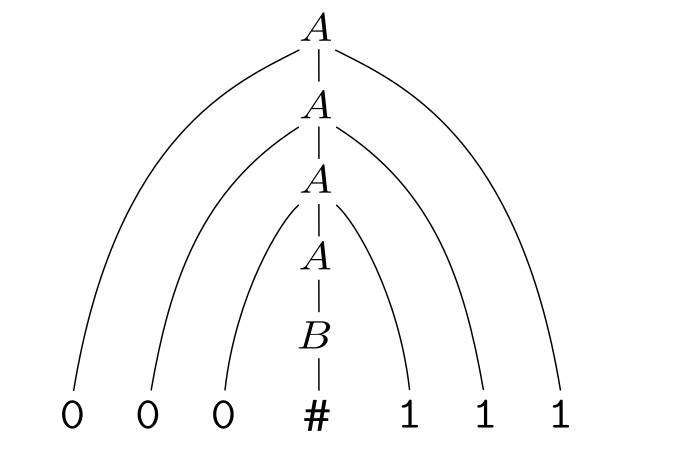
\includegraphics[scale=0.3]{figur/figur21.png}
  \end{center}
  \begin{itemize}
    \item Alle strenge der kan genereres fra \eqref{eq:cfgex} er dele af \textit{sproget af grammatikken}, som skrives $L(G_{1})$.
    \item \textbf{Ethvert sprog der kan genereres af en CFG er et kontekstfrit sprog}. (Definition, ikke sætning.)
  \end{itemize}
\end{frame}

\begin{frame}
  \frametitle{Formel Definition af Kontekstfri Grammatik}
\begin{definition}[Kontekstfri Grammatik]
  En kontekstfri grammatik er en 4-tuple $(V, \Sigma, R, S)$, hvor
  \begin{enumerate}
    \item $V$ er en endelig mængde kaldet \textit{variabler}
    \item $\Sigma$ er en endelig mængde disjunkt fra $V$, kaldet \textit{terminaler}
    \item $R$ er en endelig mængde af \textit{regler}, hvor hver regel er en variabel (venstresiden) og en streng af variabler og terminaler (på højresiden)
    \item $S \in V$ er startvariablen
  \end{enumerate}
\end{definition}
\end{frame}

\begin{frame}
  \frametitle{Kontekstfrie grammatikker, fortsat}

  \begin{itemize}
    \item Hvis $uAw$ kan blive til $uwv$, siger vi at $uAv$ \textit{giver} $uwv$, og skriver det $uAv \Rightarrow uwv$.
\item Vi siger at $u$ \textit{udleder} (ikke afleder!) $v$ hvis der eksisterer en udledning $u \Rightarrow u_{1} \Rightarrow u_{2} \Rightarrow \cdots \Rightarrow u_{k} \Rightarrow v$.
          \begin{itemize}
            \item Vi skriver dette $u \overset{*}{\Rightarrow} v$ hvis $u = v$
          \end{itemize}
    \item Sproget af en grammatik er dermed $\{w \in \Sigma^{*} \mid S \overset{*}{\Rightarrow}\}$
  \end{itemize}
\end{frame}

\begin{frame}[allowframebreaks]
  \frametitle{Tvetydighed}

  \begin{itemize}
    \item Hvis en grammatik kan generere den samme streng på mere end én forskellig måde, siger vi at strengen er afledt tvetydigt i den grammatik.
    \item Hvis en grammatik kan generere en streng tvetydigt, siger vi at selve grammatikken er \textit{tvetydig}.
  \end{itemize}

  \begin{equation}
\langle \text{EXPR} \rangle \rightarrow \langle \text{EXPR} \rangle + \langle \text{EXPR} \rangle \mid \langle \text{EXPR} \rangle \times \langle \text{EXPR} \rangle \mid ( \langle \text{EXPR} \rangle ) \mid a
  \end{equation}

  \begin{itemize}
    \item Den ovenstående grammatik er tvetydig, da den generer strengen $a+a \times a$ tvetydigt.
    \item Vi kan se dette ved at lave to forskellige parsetræer:
  \end{itemize}

  \begin{center}
  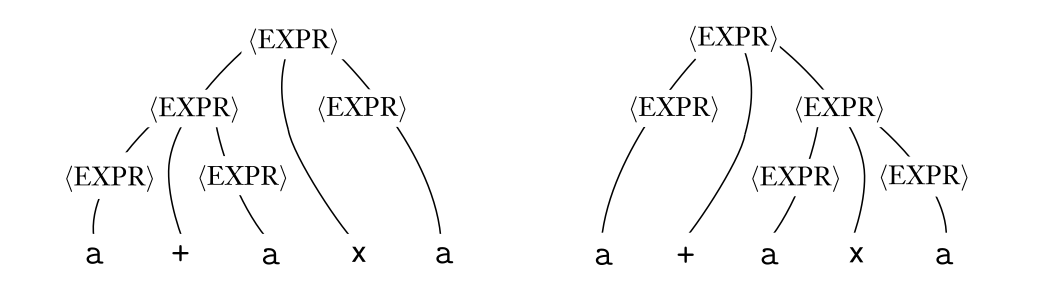
\includegraphics[scale=0.3]{figur/figur26.png}
  \end{center}
  \begin{itemize}
    \item Der eksisterer sproge der kun kan genereres af tvetydige grammatikker.
    \item Disse sprog siges at være \textit{i sig selv tvetydige}.
  \end{itemize}
\end{frame}

\begin{frame}[allowframebreaks]
  \frametitle{Chomsky Normal Form}

  \begin{itemize}
    \item (også kaldt, af Jørgen, Chomsky grammar).
    \item Chomsky Normal Form er en speciel \textit{form} til kontekstfrie grammatikker.
    \item Chomsky Normal Form sikrer nogle specifikke ting, der gør den brugbar til f.eks. algoritmer og beviser.
  \end{itemize}

  \begin{definition}[Chomsky Normal Form]
    En kontekstfri grammatik er i CNF hvis hver regel er af formen
    \begin{align*}
      A &\rightarrow BC \\
      A &\rightarrow a
    \end{align*}
    hvor $a$ er en vilkårlig terminal, og $A, B$ og $C$ er variabler, undtagen at $B$ og $C$ \textit{ikke} må være startvariablen. Vi tillader deruover også reglen $S \rightarrow \varepsilon$, hvor $S$ er startvariablen.
  \end{definition}

  \begin{theorem}
Ethvert kontekstfrit sprog er genereret af en kontekstfri grammatik i CNF.
  \end{theorem}

  \begin{itemize}
    \item Vi kan konvertere en grammatik $G$ til CNF.
    \item Vi kan gøre dette ved at, trinvist, fjerne regler der ikke overholder betingelserne, og erstatter med regler der overholder.
    \item Først tilføjer vi en ny startvariabel.
    \item Så fjerner vi alle $\varepsilon$-regler af formen $A \rightarrow \varepsilon$.
    \item Vi eliminerer også alle \textit{unit regler} af formen $A\rightarrow B$.
    \item Til sidst konverterer vi de resterende regler til den rigtige form.
\item \textbf{Bevis:}
  \end{itemize}
    \begin{enumerate}
      \item Først laver vi en ny startvariabel $S_{0}$, og tilføjer reglen $S_{0} \rightarrow S$, hvor $S$ var den tidligere variabel. Dermed sikrer vi at startvariablen ikke er på højresiden.
      \item Derefter tager vi os af epsilon-reglerne. Vi fjerner alle regler $A \rightarrow \varepsilon$ hvor $A$ ikke er starvariablen. \\ Derefter, for hver $A$ på højresiden af en regel, tilføjer vi en ny regel hvor vi fjerner $A$. Altså hvis $R \rightarrow uAv$ er en regel, tilføjer vi reglen $R \rightarrow uv$. Vi gørt dette for hvert tilfælde af $A$, så $R \rightarrow uavAw$ giver us tre regler: $R \rightarrow uvAw, R \rightarrow uAvw$ og $R \rightarrow uvw$. \\ Hvis reglen $R \rightarrow A$ eksisterer, erstatter vi denne med $R\rightarrow \varepsilon$, undtagen hvis $R \rightarrow \varepsilon$ er en regel vi allerede har fjernet. \\ Vi gentager dette indtil vi har fjernet alle epsilon-regler.
      \item Derefter fjerner vi alle \textit{unit regler}, altså for hvert $A \rightarrow B$ fjerner vi denne, og for alle $B \rightarrow u$, tilføjer vi $A \rightarrow u$, undtagen hvis dette er en regel vi allerede har fjernet, hvor $u$ er en streng af terminale og variabler. Vi gentager indtil alle unit regler er fjernet.
      \item Sidst konverterer vi alle tilbagestående regler til den rigtige form. For hvert $A \rightarrow u_{1}u_{2} \ldots u_{k}, k \ge 3$ fjerner vi denne regel, og tilføjer reglerne $A \rightarrow u_{1}A_{1}$, $A_{1} \rightarrow u_{2}A_{2}$, $A_{2} \rightarrow u_{3}A_{3}, \ldots A_{k-2} \rightarrow u_{k-1}u_{k}$
    \end{enumerate}
\end{frame}


  \frametitle{CFG Konverting Eksempel}
  Vi kigget på eksempel 2.10 pp. 110 i bogen for bedring af forståelse.
\end{frame}

\subsection{Pushdown Automater}%
\label{subsec:pda}





%%% Local Variables:
%%% mode: latex
%%% TeX-engine: xetex
%%% TeX-command-extra-options: "-shell-escape"
%%% TeX-master: "main"
%%% End:
